\chapter{Análise dos Requisitos}
O levantamento de requisitos para a construção do ePuppy foi de extrema importância, pois compreender de maneira correta e eficaz as necessidades dos usuários, é o alicerce para um sistema consistente. 
\\
\indent
Mesmo conhecendo a variedade de redes sociais disponíveis, não era o suficiente para a elaboração do projeto, por ele não se limitar apenas a uma rede social comum, mas englobar donos de animais de estimação, clínicas veterinárias, veterinários e empresas de produtos e serviços.
\\
\indent
Portanto, devido a falta de conhecimento necessário da área a ser desenvolvido o projeto, foi fundamental obter o máximo de requisitos possíveis.

\section{Elicitação de Requisitos}
Por conhecer bem que o levantamento de requisitos não é uma tarefa fácil, devido a dificuldades que os usuários tem de descrever o problema ou até mesmo, pela possibilidade de haver contradições de ideias entre usuários e analistas, utilizou-se técnicas padrões usadas na Engenharia de Software. Abaixo, seguem algumas das técnicas utilizadas na elicitação dos requisitos:
\begin{itemize}
   \item Entrevistas com usuários:
   \\
   \indent
   Por ser um método tradicional e que geralmente constrói bons resultados, os mais variados tipos de usuários foram entrevistados, principalmente, veterinários e donos de animais. 
   \item {\it Brainstorming}:
    \\
   \indent
   O {\it Brainstorming} foi outro método utilizado e que também rendeu bons resultados. Foi realizada principalmente entre veterinários, pois poderiam contribuir da melhor forma possível, por viver no ambiente cotidianamente. 
   \item Estudo Etnográfico:
   \\
   \indent
   Em conjunto com os {\it Brainstormings} e entrevistas com usuários, realizamos o estudo baseado na observação, para compreender o ambiente e o contexto onde o sistema será inserido.
   \item Prototipagem: 
   \\
   \indent
   Para a demonstração do andamento do projeto, apresentamos protótipos com algumas funcionalidades, principalmente para as clinicas e veterinários, para que essas começassem a se familiarizar com o sistema e divulgá-lo aos seus clientes.
   \item Workshops de requisitos:
   \\
   \indent
   Além de todos os métodos que utilizamos anteriormente, também realizamos várias reuniões estruturadas com veterinários, clinicas e investidores, a fim de modificar, adicionar ou esclarecer os requisitos.
 \end{itemize}
 
 \section{Diagrama de Casos de Uso}
Os casos de uso descrevem as principais funcionalidades do sistema e a interação dessas com os demais usuários, não aprofundando em detalhes técnicos, ou seja, não descreve como o sistema realiza tais funções.
\\
\indent
A partir dos casos de uso, podemos identificar uma sequência de eventos que acontece quando um usuário interage com o sistema (Cenário), usuários do sistema (Atores), funcionalidades realizadas pelos atores ({\it Use Case}) e a comunicação, que será basicamente o que liga um ator a um caso de uso. Abaixo, estão demonstrados os casos de uso, subdivididos em módulos:


\begin{figure}[h!]
	\centering	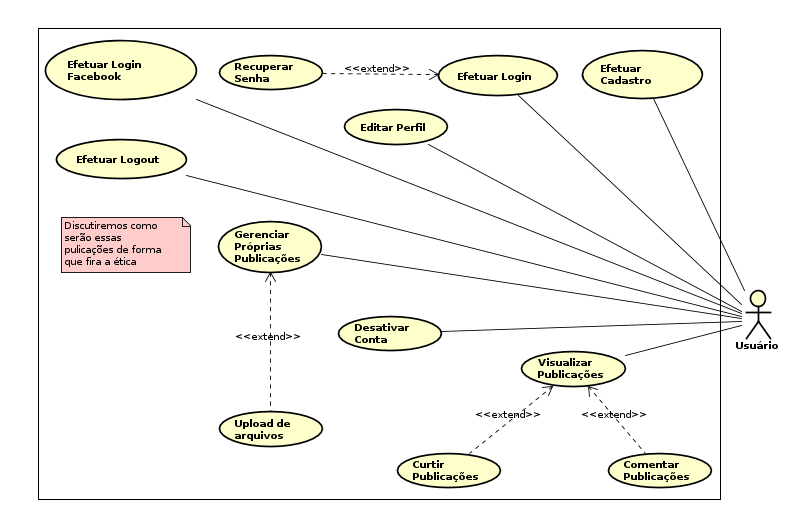
\includegraphics[scale=0.55
	]{imagens/usercasodeuso}
	\caption{Módulo usuário}
	Fonte: Autoria Própria.
	\label{Rotulo}
\end{figure}

\begin{figure}[h!]
	\centering	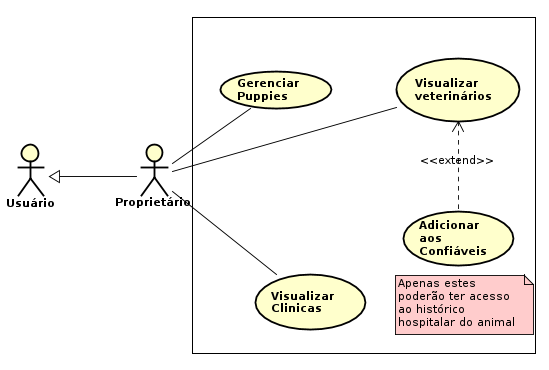
\includegraphics[scale=0.55
	]{imagens/ownerscasosdeuso}
	\caption{Módulo Proprietário}
	Fonte: Autoria Própria.
	\label{Rotulo}
\end{figure}

\begin{figure}[h!]
	\centering	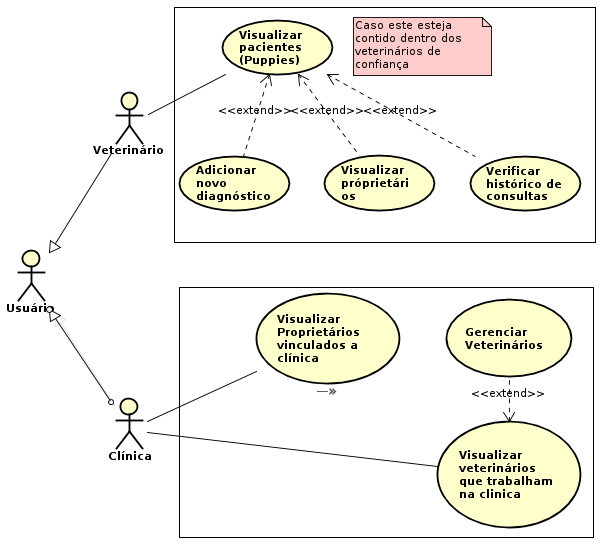
\includegraphics[scale=0.55
	]{imagens/HeVcasosdeuso}
	\caption{Módulos Veterinário e Clínica}
	Fonte: Autoria Própria.
	\label{Rotulo}
\end{figure}

\newpage

\section{Diagrama Entidade-Relacionamento}
O Diagrama de Entidade e Relacionamento descreve toda estrutura lógica do banco de dados,  ou seja, represente de forma abstrata a estrutura que possuirá o banco de dados da aplicação.
\\
\indent
A partir de modelo pode-se descrever os objetos (Entidades) envolvidos em um domínio de negócio, suas caraterísticas (atributos) e seus relacionamentos.

\begin{figure}[h!]
	\centering	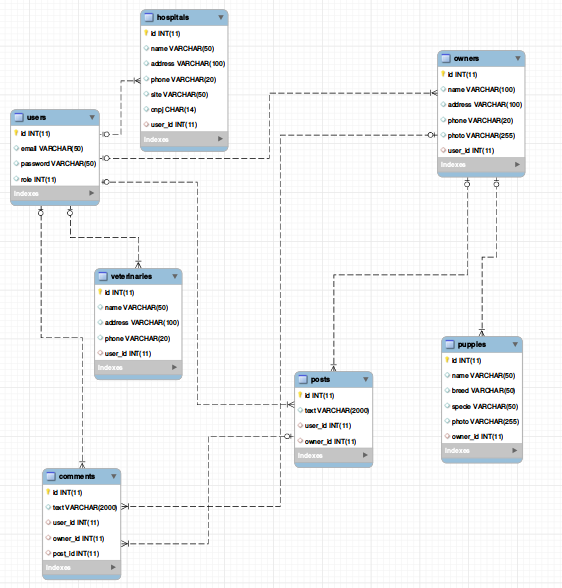
\includegraphics[scale=0.80
	]{imagens/entidaderelacionamento}
	\caption{Diagrama Entidade-Relacionamento}
	Fonte: Autoria Própria.
	\label{Rotulo}
\end{figure}
